%!TEX root = ../main.tex
% file: assignment2.tex

\graphicspath{{C:/Local_Files/GitHub/MCS507_Final_Project/tex/include/}}
%\graphicspath{{C:/Documents and Settings/amcelhinney/My Documents/GitHub/MCS507_Final_Project/tex/include}}
%\graphicspath{{C:/Documents and Settings/amcelhinney/My Documents/GitHub/MCS507--Project-3/tex/include/}}

\section{Assignment Two: Overview of the $Orange$ Software Package} % (fold)

\subsection{About $Orange$} % (fold)

\begin{flushleft}Bayesian Classifiers may be used in Python via the $Orange$ modules. However, $Orange$ is actually a comprehensive data mining suite with capabilities far beyond just one classifier.
\end{flushleft}

\begin{flushleft}The stated goal of $Orange$ is \quote{...not to cover just about any method and aspect in machine learning and data mining (although through years of development quite a few have been build up), but to cover those that are implemented deeply and thoroughly, building them from reusable components that expert users can change or replace with the newly prototyped ones.} 
\end{flushleft}

\begin{flushleft}To accomplish these goals, $Orange$ developers refer to a ``component-based framework". The three components of this framework are:
\end{flushleft}
\begin{enumerate}
\item A library of C++ core objects and routines
\item A collection of Python modules that site over the core library
\item A collection of graphical widgets that are implemented via a visual programming framework
\end{enumerate}

\begin{flushleft}
$Orange$  is developed by the Artificial Intelligence Laboratory in the Department of Computer and Information Science in the University of Ljubljana, Slovenia ($Orange$ Documentation, 10/20/2012). The suite was the realization that several researchers at the laboratory were each independently writing their own code for scoring, model building etc. $Orange$ was accepted into the Google Summer of Code Project in 2012 which resulted in the creation of the following projects:
\end{flushleft}
\begin{enumerate}
\item Widgets for statistics
\item Computer vision add-on for $Orange$
\item Multi-Target Learning for $Orange$
\end{enumerate}

\begin{flushleft}$Orange$ features implementations of the majority of cutting-edge machine learning and data mining techniques, including techniques from the following categories:
\end{flushleft}

\begin{enumerate}
\item Summary Statistics
\item Classification
\item Regression
\item Ensemble Algorithms
\item Clustering
\item Network Analysis
\end{enumerate}

\subsection{Overview of the $Orange$ GUI}

\begin{flushleft}$Orange$ features a GUI with a unique visual programming paradigm. Visual programming refers to the collection of widgets which are implemented on a visual canvas. These widgets are modular pieces of code that are manually dragged by the user onto the canvas. 
\end{flushleft}

\begin{figure}[H]
    \centering
       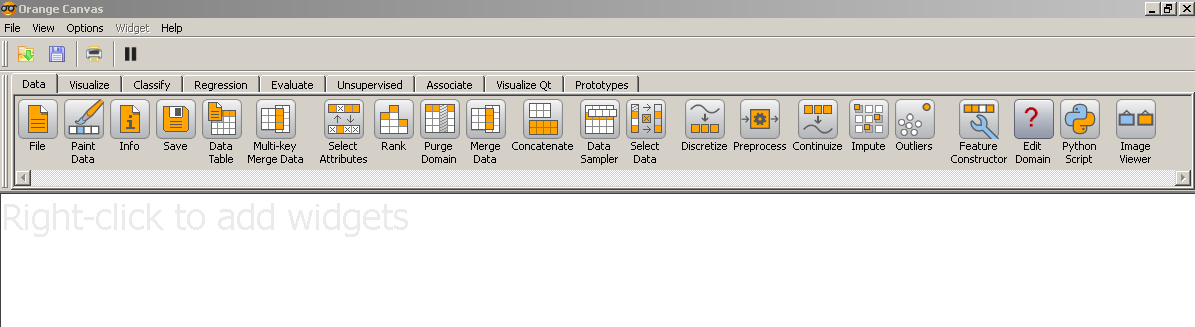
\includegraphics[width=6.5 in]{orange_canvas.PNG}
    \caption{Image of the $Orange$ Canvas with Widgets Displayed at Top}
\end{figure}

\begin{flushleft}Each widget performs a discrete action and contains a set of inputs and outputs. Hovering over a widget reveals its inputs and outputs. \end{flushleft}
\begin{figure}[H]
    \centering
       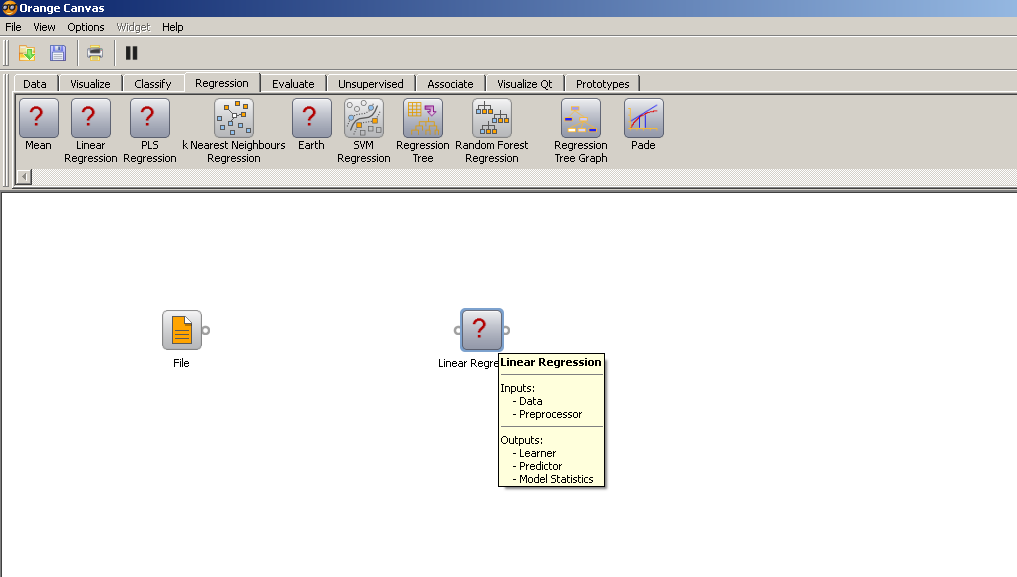
\includegraphics[width=6.5 in]{orange_widget_features.png}
    \caption{A Widget Displaying its Inputs and Outputs}
\end{figure}
Then a widget with an output equal to the input of another widget can be combined by the user dragging a line from the one widget to the other. In this way, the user is ``programming" without writing any code. Additional options for each widget can be found by clicking on the widget while it is placed on the canvas.
\begin{figure}[H]
    \centering
       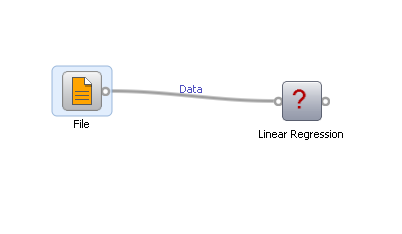
\includegraphics[width=3.5 in]{orange_connection.PNG}
    \caption{Connecting Widgets}
\end{figure}

\begin{flushleft}$Orange$ claims that the user should be able to complete a sophisticated data mining project entirely using the canvas. However, in my experience it seems like supplemental Python knowledge would definitely be required. Particularly if one wanted to complete more sophisticated data cleaning or graphing than are supported by the canvas. However, the canvas definitely can be used to supplement the code. 
\end{flushleft}



